\section{Introduction to the project}
At the time of writing, I have been working for the company for over a year on their financial wellbeing platform. The purpose of the platform is to help users connect with coaches and give them tools to educate themselves, get their finances under control and plan for the future.

This project has been in development for over 4 years with only a handful of developers. The backend is written using microservices architecture in Rust and there are 2 frontend applications: native iOS and web. There are also two additional web frontends for administration. Admin portal is used by financial advisors to communicate with users and also by support/admin users. The latter is the customer portal, available to our customers (employers) to see their employees' interactions with our platform.

Over the years the platform has gained a lot of features, so I will just highlight the main ones to give you an idea of what the platform does. I will describe the processes using user journeys:

\begin{example}[Sign Up]
    Joe, an employee of company Z, receives an email about gaining access to the platform, which his employer has purchased as a benefit. Joe opens a web browser and goes to the registration page. He enters his email and password and goes through the onboarding process (a few basic questions about his financial experience and goals). Once registration is complete, he lands on the home page.
\end{example}

\begin{example}[Advisor]
    Immediately after signing up, Joe is presented with the name of his personal financial advisor. He can send him a message via chat, or better still, schedule a phone call so they can meet face-to-face, get to know Joe's expectations, review his finances and set some goals.
\end{example}

\begin{example}[Analyse]
    Meanwhile, as Joe waits for his first meeting with his adviser, the platform offers to connect his bank accounts so it can give him some insight into his spending. In the UK, there is an open banking standard that allows him to give the application access to his accounts and transactions in just 3 steps. Once connected, Joe is presented with graphs showing how much he spends each month in each category. He can also set goals (e.g. wedding or buying a house), link them to accounts and it will automatically track any progress (savings).
\end{example}

\begin{example}[Education]
    On the Learning page, Joe can read thousands of financial articles written by our financial advisors or watch recordings of past webinars. He can also view and register for upcoming webinars.
\end{example}

% \subsection{Vocabulary}
% Before moving into technical side of the thing, we need to first define few terms, which will be used throughout this chapter:
% \begin{description}
%     \item[Insight]
% \end{description}


\section{Infrastructure}
The infrastructure is based on HashiCorp products (HashiStack). A cloud provider is used for VM provisioning and networking, but they manage the rest themselves via custom Terraform scripts (IaaS). What are the key components:
\begin{itemize}
    \item \it{Nomad} is a simple and flexible scheduler and orchestrator for deploying and managing containers. \cite{NOMAD}
    \item \it{Consul} is a service networking solution that automates network configuration, service discovery and secure connectivity. \cite{CONSUL}
    \item \it{Vault} secures, stores and tightly controls access to tokens, passwords, certificates, API keys and other secrets critical to modern computing. \cite{VAULT}
\end{itemize}

I don't know what the reason was for going with the HashiCorp stack, but looking at the experience with it after a year, I'm amazed at how well the components integrate, and the setup/management of the whole cluster was a breeze compared to Kubernetes (K8s). There are now many managed K8s clusters available, but not a single managed Nomad cluster provider that I could find (there was an unmanaged.io project, but it seems to be down). I think the reason for this is simple - Nomad is just easy to run and manage. I'm not condemning K8s, I'm sure the complexity is there for a reason, but just for this project Nomad was more than enough and much easier to work with. During the year we had 2 incidents in production. The first was caused by a weird cluster state, which was resolved by rebooting, and the second was caused by our cloud provider having network issues. As we had no one dedicated to infrastructure and everything was managed by the BE developers, we just needed something that was easy to use and would work. Nomad did exactly that without adding any complexity that we did not need and that K8s would most likely add.

Even though this is a relatively simple microservices infrastructure, it still consists of a lot of components that new developers needed some time to get used to. A few examples:
\begin{enumerate}
    \item The API gateway was created using a proxy called \textit{fabio}, which has it's own way of defining path mapping.
    \item Nomad has it's own job definition language called HCL.
    \item The inter-service communication needs to be protected because it is over the network. So additional secrets handling and service discovery had to be done before each inter-service call.
    \item Changing deployment properties requires vast knowledge of devops and editing quite complex pipelines.
\end{enumerate}
None of the above examples of obstacles exist when working with monoliths.



\section{Microservices architecture}
The whole platform consists of 26 microservices, 4 of which are backend for frontend. Each microservice exposes its API via HTTP protocol for inter-service communication as well as to the outside world and API Gateway is created via reverse proxy called \textit{fabio}. For background tasks, a messaging system with queues is used, specifically Amazon's SNS for sending messages and SQS for receiving them.

Git is used for versioning with one repository per microservice. I see some advantages in having separate repositories compared to monorepo. Firstly, pull requests are better organised and compact - changes to a microservice should be isolated, and having Monorepo allows code in multiple microservices to be touched, and it would be up to the code reviewer to notice. It also forces developers to think of changes as more isolated, since they can only change a single microservice in a single repository - they have to switch to another to make the next changes. The same flow could be enforced by git hooks, for example, but this way it requires no configuration. On the other hand, it is a bit harder for newcomers to simply download all repositories, as 26 is quite a lot and requires some structure to be added to local repositories for easier navigation.

Finding the right size of microservices is a difficult task. In this project, the domain driver approach was used to find 'small enough pieces' (this was an approximation) and map them into microservices. Some have well-defined boundaries, some have a gray area, few are overgrown and should have been split because maintenance has become much harder with increasing complexity. A few examples:

\begin{itemize}
    % TODO add more examples
    \item \it{Financial Account} holds information about bank accounts for users. Either manually created accounts or those that are connected with bank.
    \item \it{Transaction} stores financial transactions.
    \item \it{Categorisation} contains pure logic that categorises transactions into different categories.
    \item \it{Orchestrator} is used for scheduled tasks that trigger complex flows involving multiple microservices, such as updating cached accounts and Open Banking transactions, and starts the post-processing.
    \item \it{Advisor} was designed to hold the logic and data around advisors and their relationship with users. Later, chat functionality was added, and as it started with just basic messaging between advisors and users, the unfortunate decision was made to include everything around messaging here as well. Over time, this functionality has been extended and this microservice has become the most bloated of all.
\end{itemize}

From the examples above, it is clear that microservices have varying scopes/boundaries. Even if we have the best possible design at the start, over time, features will change and this will inevitably lead to an uneven distribution of boundaries. This does not mean that there is a problem with the design, as our system might just be adapting to our changing business needs, shifting goals, and our design needs to adapt as well. There are usually two outcomes. The first is a proper adaptation of the design, once we realise that the change is needed, and with it a possible refactoring/split/merge of microservices. The second option is what happened to the Advisor service. Over time, it took on more and more functionality, even outside its scope, and when someone later realised the mistake, the amount of work required to make the necessary changes was simply too much to invest at the time.
% how is this possible? Microservice from definition is independent and isolated, so it should be easy just to split into two. Well, even though definitions sound great, the complexity always depends on the actuall implementations. 
% - contracts (swaggers)
% - compatibility
% ability to remove something from contract
% tracking dependency

\section{Characteristics}
This section describes the project along the same lines as the architectures compared in the
chapter~\ref{chapter:architectures}.

% TODO popsat deployment complexity
% Popsat stroze flow, víc to rezipíšu obecně v Analyse chapter
\subsection{Performance}
In terms of performance, there were only two services that had noticeable CPU usage and those were processing thousands of financial transactions every time the user opened the analysis page, the rest was mainly waiting for the database to read or write data. Despite this, we had very linear traffic and each service was only running in two instances with no autoscaling and only a few hundred MHz of CPU allocated to it, so it was almost like Monolith with two instances, with the exception that even internal requests were load balanced and not just external as with Monolith. So in this case, it would easily run as a monolithic system without any problems, with plenty of room to grow vertically: with 26 microservices, each would have 500\.HMz of CPU and 100\.MB of memory allocated. The total resource requirement for a single monolithic instance would be 5~CPU cores (2\.GHz per core) and 1\.GB of memory.

\subsection{Maintanability}
% TODO it gets complicated - need to expose lot of APIs (+ maintanance), hard to solve security 
The idea of having lots of micro independent services is great from a scaling and rapid deployment perspective, but as with everything, there are negatives. Each service defines its own interface, in this case as a Swagger definition, and is kept in sync with the code manually, which inevitably leads to problems. There are some automated solutions that either generate the OpenApi definition from the code or vice versa. Unfortunately, it has some limitations, not every language has support for it, and I have not seen any project that actually uses it and relies on it completely. These outdated contracts have led to confusion for front-end developers, an inability to rely on it, and in practice, every time a front-end developer needed detailed behaviour about an endpoint, he had to contact a back-end developer who would investigate the behaviour directly from the code. Today, gRPC technology would probably be better for inter-service communication, as it has support for every major language and can automatically generate either server or client implementations from schema.

\subsection{Sustainability}
Defined contracts, whether via OpenApi or any other technology, ideally need to be maintained indefinitely, which is of course not possible. Even with the best design in mind, requirements will change, features will become obsolete, and maintaining each obsolete/old/unused feature will take a lot of time. In monolithic/modular statically typed systems, when someone changes the interface/contract, the compiler gives instant feedback as to whether these changes can be made, or whether there are conflicts, and where exactly. In the world of microservices, this is a much more complex issue. Taken to the extreme, each service implements its own client to communicate with all dependent microservices. When this happens, as it did in this project, how can you tell if even a specific change as small as removing a single field on the contract will affect other microservices, if any? Perhaps using an advanced static code analysis tool for this specific purpose would give an idea, but I doubt it would be reliable. Another option I took after seeing this, also code duplication with this approach, was to publish the client implementation with each contract change. That way, other microservices could simply add the client library as a dependency instead of implementing their own. Tracing dependencies between services was now as simple as checking dependencies and looking for client libraries. Now at least the incompatible changes to contracts are at least somewhat possible, as a new version of the client library can be released and each microservice can be rebuilt (e.g. as part of CI) with the updated client library to see its impact.

\subsection{Testability}
The worst part on this project was, and most likely is with every microservices project, the inability to properly check if all the contracts for each service are fully compatible, or if there is simply a typo somewhere, or if during refactoring a service was simply left out, which actually happened here from time to time. Even though we had the code coverage, the tests were still expecting the older version of the contract, so the problem would show up once it was running in the real environment. At best, we would catch it in development, at worst it would show up in production after release.

\subsection{Complexity}
Leveraging our existing code convention across services, I was able to generate a dependency graph for the whole system via static analysis, see graph \ref{img:microservices-current-commented} (something that was not available and no one paid attention to). This is a real example of what can happen to a microservices architecture after 3 years of development, and this graph does not include communication via async messages. It is not easy to say whether the state looks bad or not, but I would lean towards bad after seeing the graph. If this were the module dependency graph of Modulith, it would take some time to make changes, but once done and the compiler was happy, it would be done. But if someone wants to do these big kind of changes like change contracts (internal just between services) in microservices it is much more work having to change contract, client implementation, propagate the change to every service where it is used. Just to see where it is used is a task on its own compared to a single process system where every IDE is fully capable of showing you in a matter of seconds every single usage in the codebase.


\begin{figure}
    \centering
    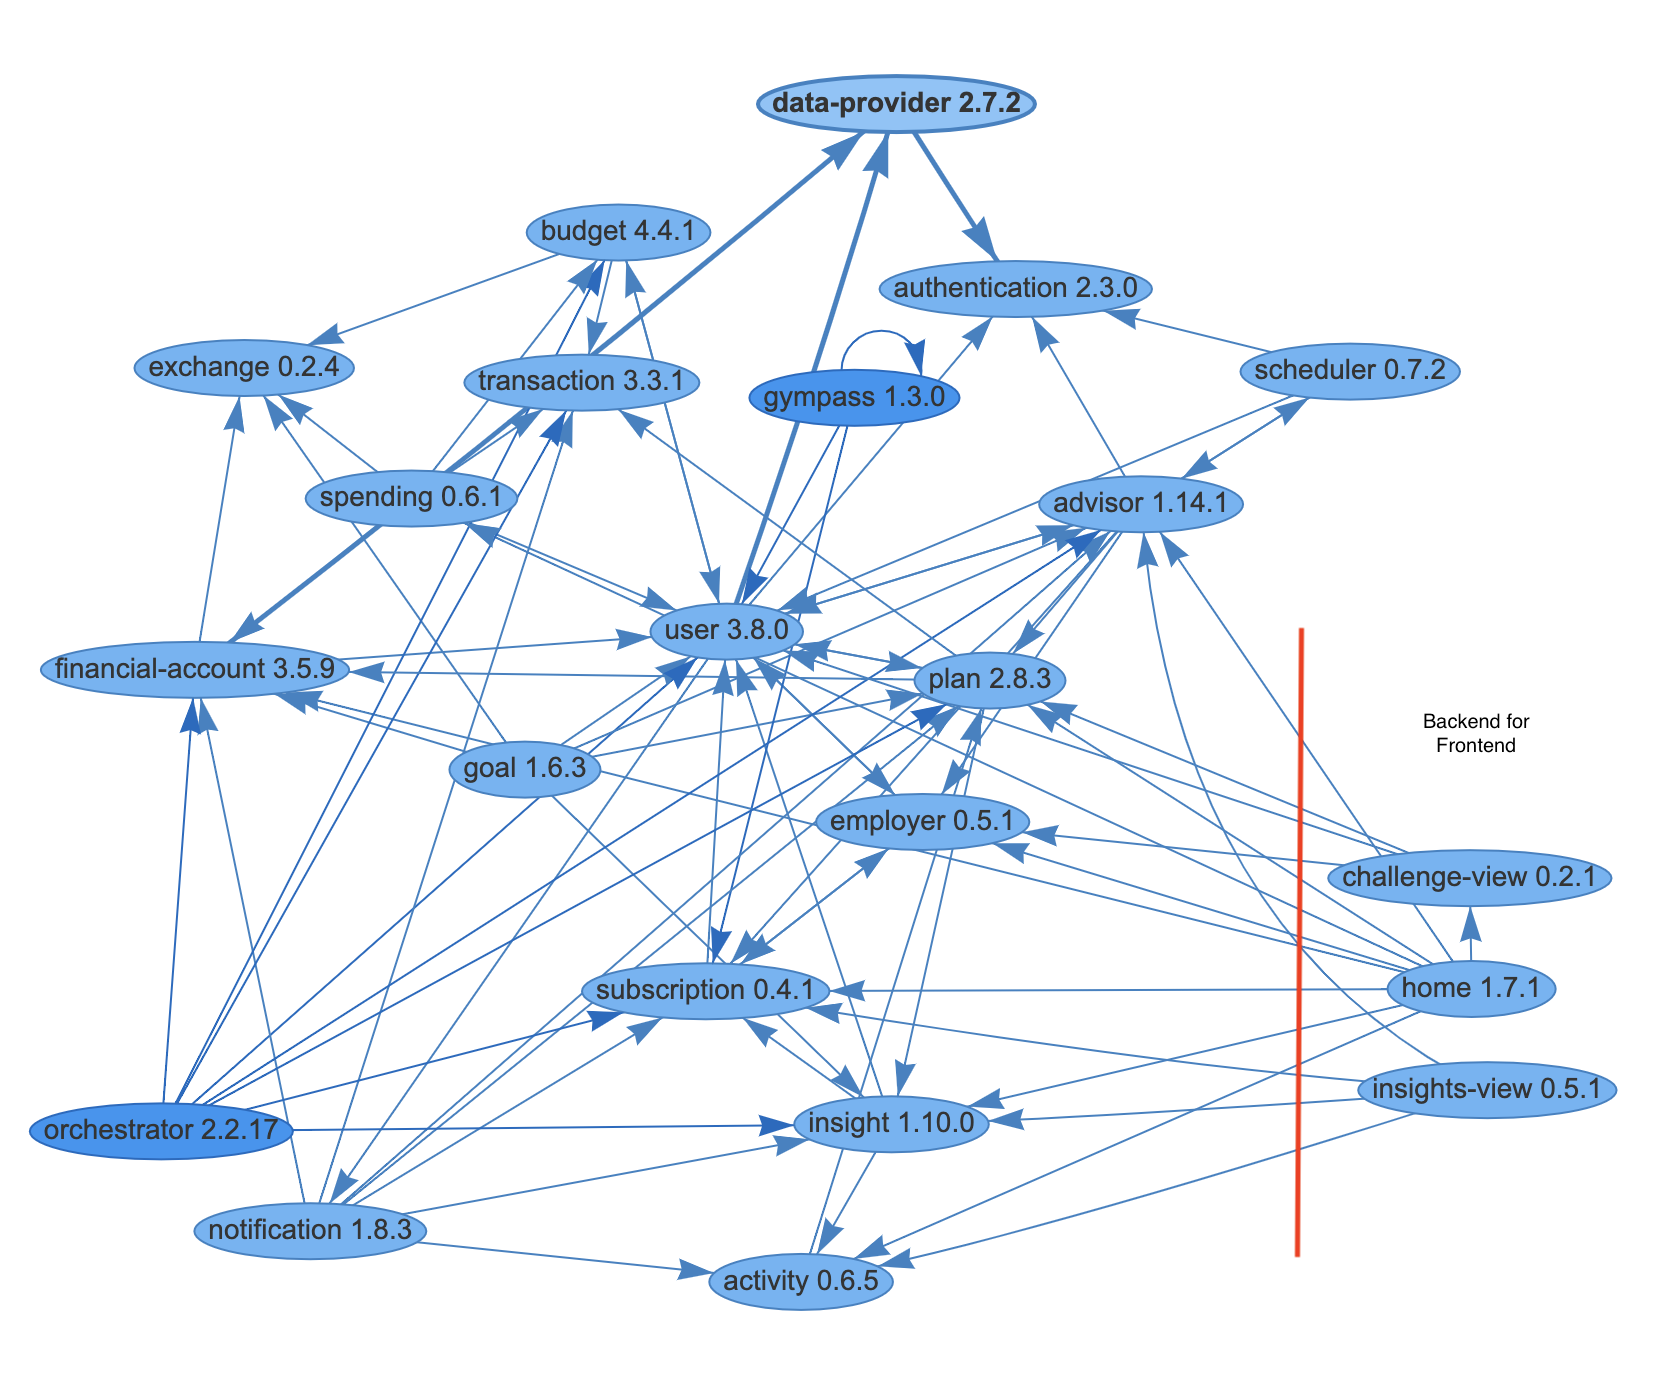
\includegraphics[width=\textwidth]{images/microservices-current-commented.png}
    \caption{Inter microservice dependency graph of backend after roughly 3 years of development. \label{img:microservices-current-commented}}
\end{figure}

\section{Summary}
The author describes his personal experience with a microservices project, highlighting the added complexity of the chosen microservices architecture and how intertwined individual services can become, despite the architecture promising low coupling. Because one thing is the ``feature'' of the architecture, and quite another is how well it is actually implemented and maintained over the years of development.


% Working on bigger feature it meant touching multiple services. Later the deployment required to check all not-deployed work and figuring out what has been tested and can be deployed to production. This flow is most likely the same for all projects, just for Microservices it is easier compared to Monolithic since the change are usually much smaller.

% \section{Personal project}
% In spare time I am working on personal Internet of Things platform project (repository located at \href{https://github.com/founek2/IOT-Platform}{https://github.com/founek2/IOT-Platform}). Although I am only working on it solo, it has become quite a complex solution over the span of 5 years. The platform consists of a backend, a website as a multiplatform frontend, a library for embedded devices, bridges for third party devices and it is integrated with MQTT broker for communication and the automation tool node-red for defining visual flows. In 2021 I wrote my bachelor thesis completely based on this project and later I split the backend into multiple services, effectively migrating from monolithic architecture to microservices.

% The reason behind the migration at that time was to introduce some boundaries between different parts of the application. The backend consisted of 3 microservices. The \textit{Authentication} microservice handled passwords, tokens and access control. The second microservice was subscribed to the MQTT broker and stored all changes in a database and sent commands to the devices. And the third was the biggest, as it implemented most of the API exposed to the front-end (it consisted mainly of simple CRUD operations).

% Unfortunately, the migration has a lot of negative effects, so I recently decided to migrate the architecture to Modulith. The problems:
% \begin{itemize}
%     \item Deployment complexity - the whole application is designed to run in a single instance, so it was deployed via Docker, specifically `docker-compose' yaml file, which was very simple definition for single container (not mentioning other containers like database). After the migration, I decided to still use a single docker image for all services, as this would keep the build process simpler. But the `docker-compose' file now grew almost 3 times, as two additional containers now had to run with partially duplicate definitions for environment variables and mutual references.
%     \item Complicated development - previously to run the whole application it was just a matter of running 2 commands to run the frontend and backend. Now the backend has been split into 3 services, so it was a matter of running 4 commands. It would be possible to use a process manager like \textit{pm2}, but it requires knowledge of the tool to be effective with it, and I wanted to keep it as simple as possible, so I ran each command in a separate terminal where the logs were easily visible. Distributed tracing and logging was not necessary as there are only 3 inter-service network calls. But most of the time, if something went wrong, it was just a lot harder to find the log in the first place, as there were now 3 places to look instead of just one. Later on, I often found myself rejecting the idea of implementing additional functionality because it was just too painful to set up the environment I was not working with on a day-to-day basis. And this is where I see the biggest problem. As soon as the architecture starts to get in the way of an effective development process, we should start to ask ourselves whether it is bringing more benefits or negatives. And in this particular application it has been the former.
%     \item Distributed system - even though the whole application is designed to run in a single instance, with microservices we always get a distributed system, and implementing any shared state becomes quite a challenge. Recently I decided to finally implement some advanced login token management functionality. Previously there was no control over how many devices or which ones were signed into the user account, so it was impossible to cancel the user session if it was hijacked. I implemented a new login procedure and needed a way to invalidate the JWT token. Since each service validates the token on its own through public key, because for this routing all to authentication service would add a lot of latency, I needed some shared state where I can mark which tokens are no longer valid. With monolith it would be simple as having a single shared object and each service would cryptographically validate the token and also check the shared object if the token was not invalidated. Unfortunately, I had the microservices and adding shared state to a distributed system is a complex task (it also needed to be fast as the validation is done on every request). One solution would be to introduce an in-memory database to hold the shared state, and the services would query the database on each token validation.  But again, this adds an unnecessary amount of complexity - a new database to host, learn the language, maintain connections. When all this could have been easily solved with a single shared object, which is possible in Modulith.
% \end{itemize}